\documentclass[11pt]{amsart}
\usepackage[top=0.75in,left=0.75in,right=0.75in,bottom=0.75in]{geometry}                
\usepackage{amssymb,amsmath,graphicx}

\newcommand{\ff}{\mathbf{f}}
\newcommand{\bx}{\mathbf{x}}
\newcommand{\bv}{\mathbf{v}}
\newcommand{\bu}{\mathbf{u}}
\newcommand{\bt}{\mathbf{t}}


\begin{document}
	
	\section*{Two bead model}
	
	A microorganism that is propelled forward by the motion of a flagellum at its tail is called a pusher. The far field flow around a pusher looks like a dipole. An approximation to a dipole is two forces separated by a small distance $\ell$ which are equal in magnitude but opposite in direction, $\ff$ and $ -\ff$. The forces are not only parallel, but positioned in a colinear fashion -- the forces are in the direction of the vector connecting their locations $\bx_h$ and $\bx_t$. One can think about each of these forces coming from spheres of radii $r_h$ and $r_t$ at the head and tail of an organism. If the spheres have equal radii, then no propulsion can occur. If the radii are nonequal, then the differential drag on the spheres will cause motion in the direction of the body orientation $\bv = \bx_h-\bx_t/|\bx_h-\bx_t|$. The smaller sphere (head) will be propelled away from the larger sphere (tail).
	
	\begin{center}
	\begin{tabular}{c}
	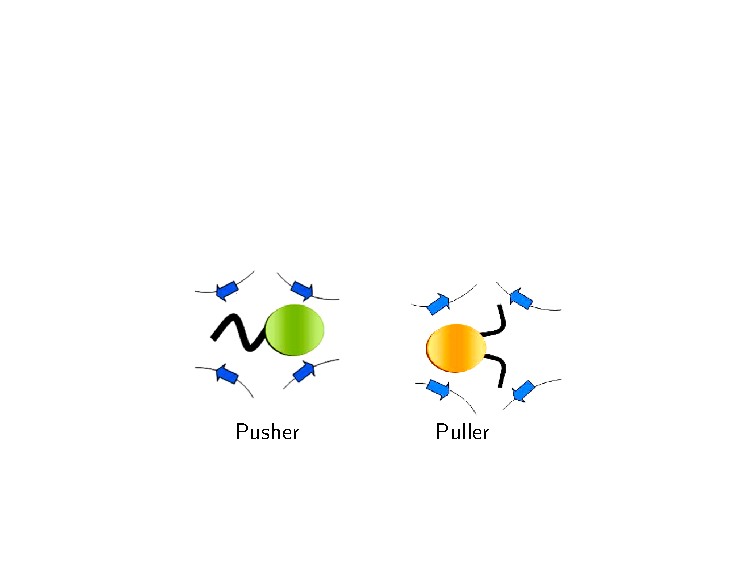
\includegraphics[width=4.0in]{PushersPullers.pdf} \\
	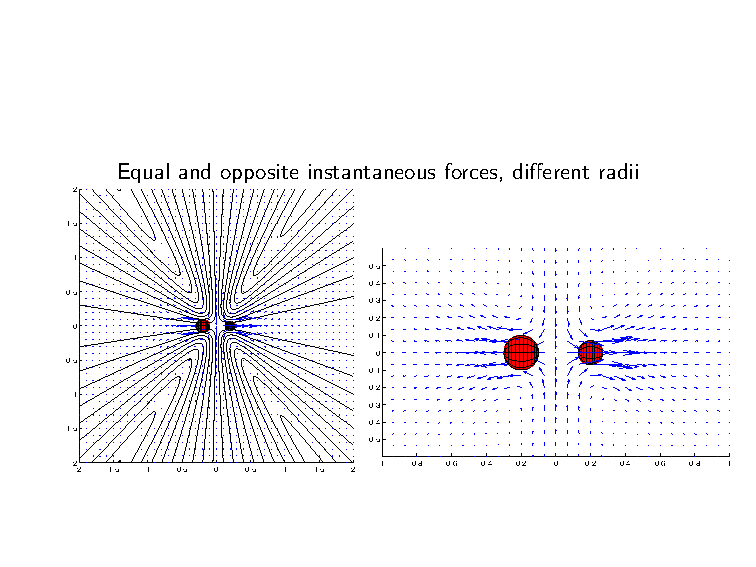
\includegraphics[width=5.0in]{TwoSphereDipole.pdf}
\end{tabular}
\end{center}
	
	Usually in a two-bead model of an organism, steps are taken to ensure that the beads remain together. This may be accomplished by adding additional forces, commonly spring forces, but also forces that help ensure that the head and tail beads move at the same velocity as each other in the absence of other simulated organisms. Shilpa and Ricardo kept the two points together by using regularized Stokeslets instead of spheres and taking a limit as $\ell \to 0$. In these cases it is necessary to have an equation for body orientation.
	
	\begin{center}
	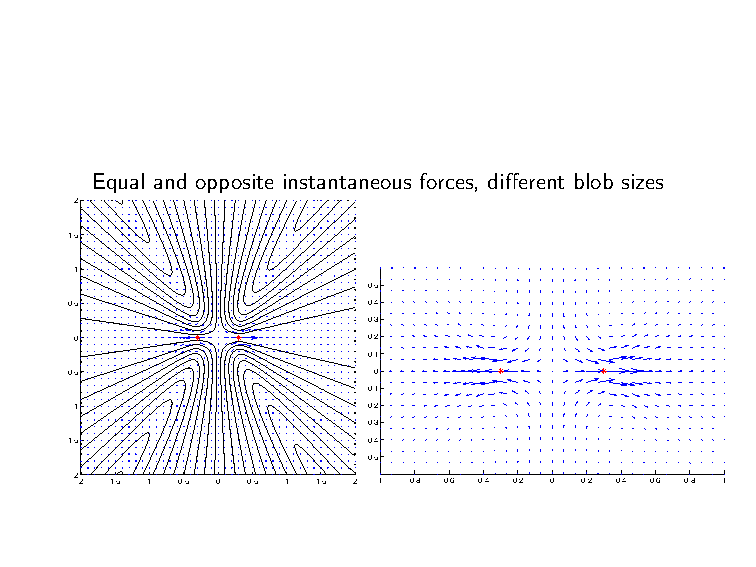
\includegraphics[width=5.0in]{TwoBlobDipole.pdf}
\end{center}
	
	For our model, we will also use regularized Stokeslets, but we will not try to keep the beads together. Instead, we will consider the tail bead a ghost bead that provides the correct far field velocity and body orientation at each moment in time, but we will not constrain its velocity. At each time step, we will reinstate the ghost tail bead at the proper location. If there is only one swimmer, then the body orientation will never change because the forces are colinear with the body axis. Our algorithm is demonstrated pictorially below.
	
	\begin{center}
	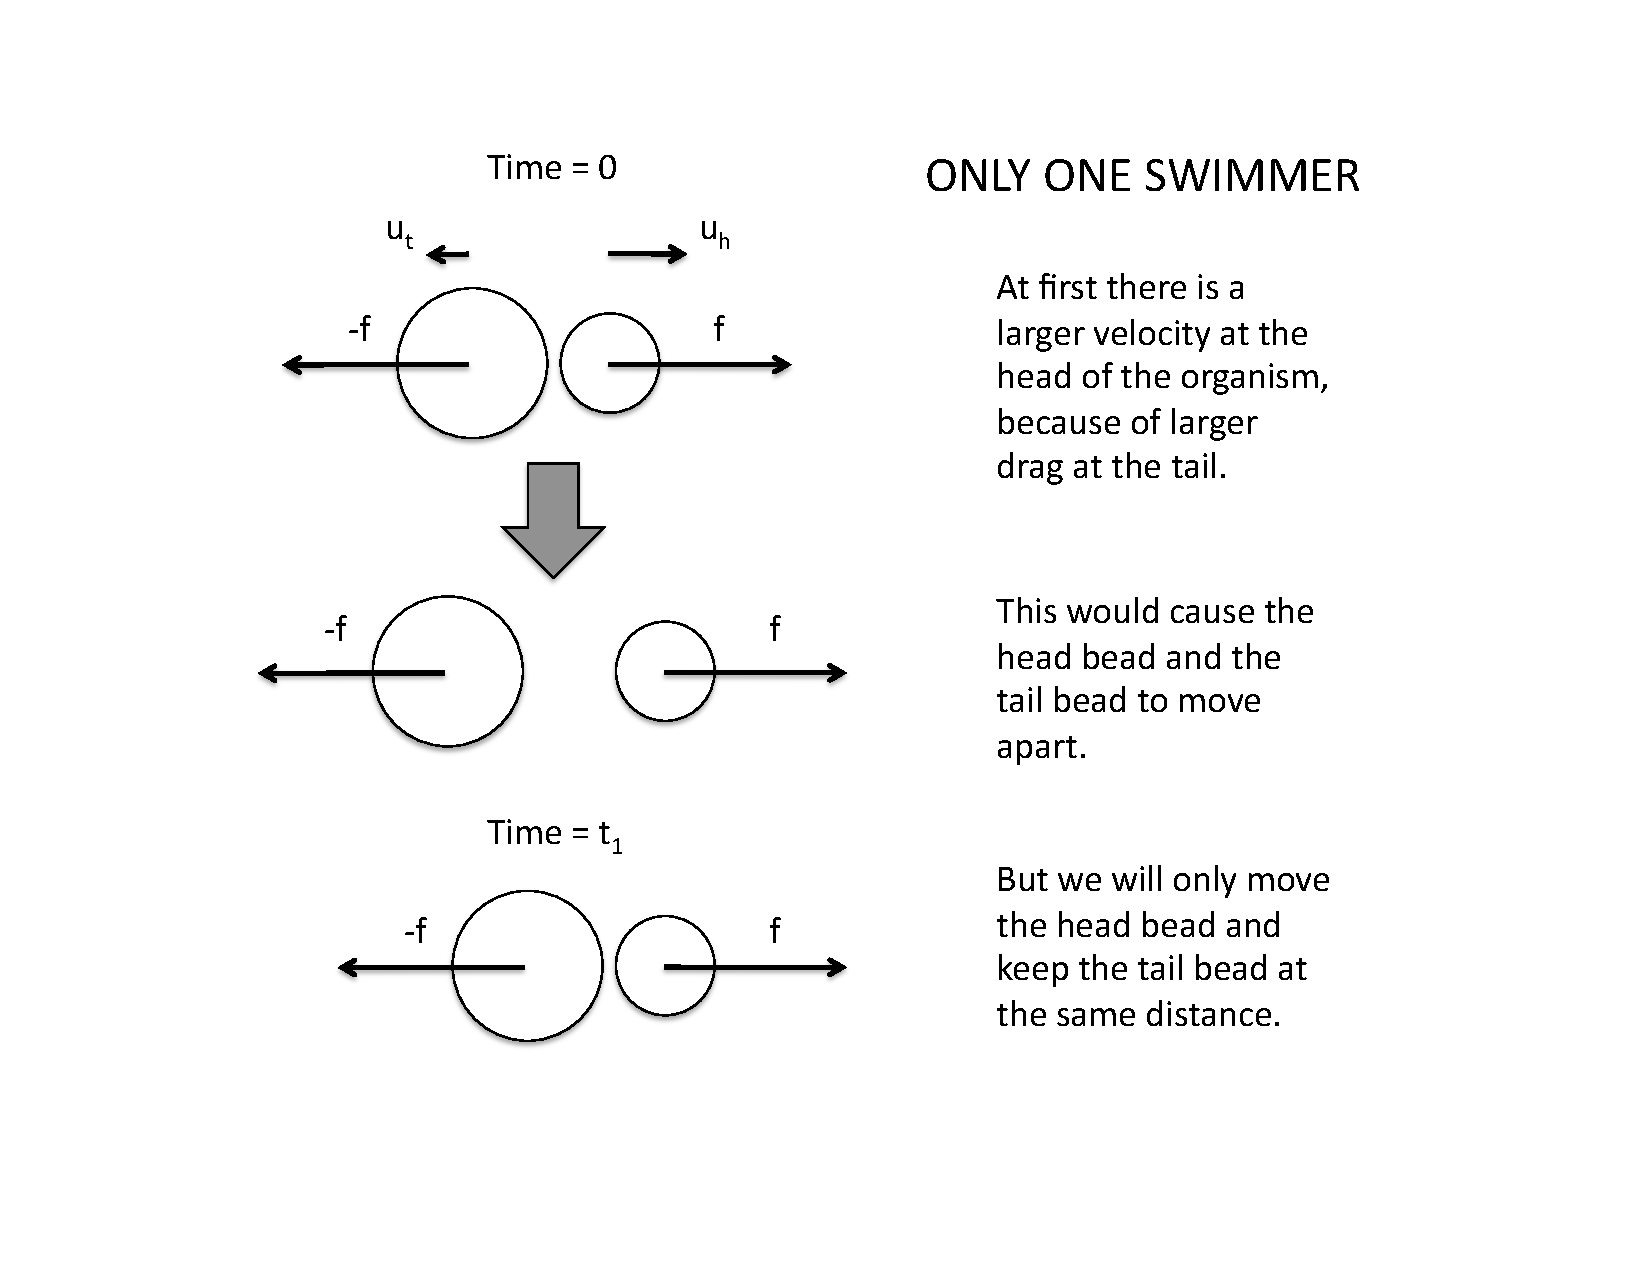
\includegraphics[width=6.5in]{SingleSwimmer.pdf}
\end{center}
\pagebreak

	If there are multiple swimmers, then the additional forces can cause changes in body orientation. We use the ghost point to track the change in orientation, and when we update the ghost point position, we also update the direction of the forces.

	\begin{center}
	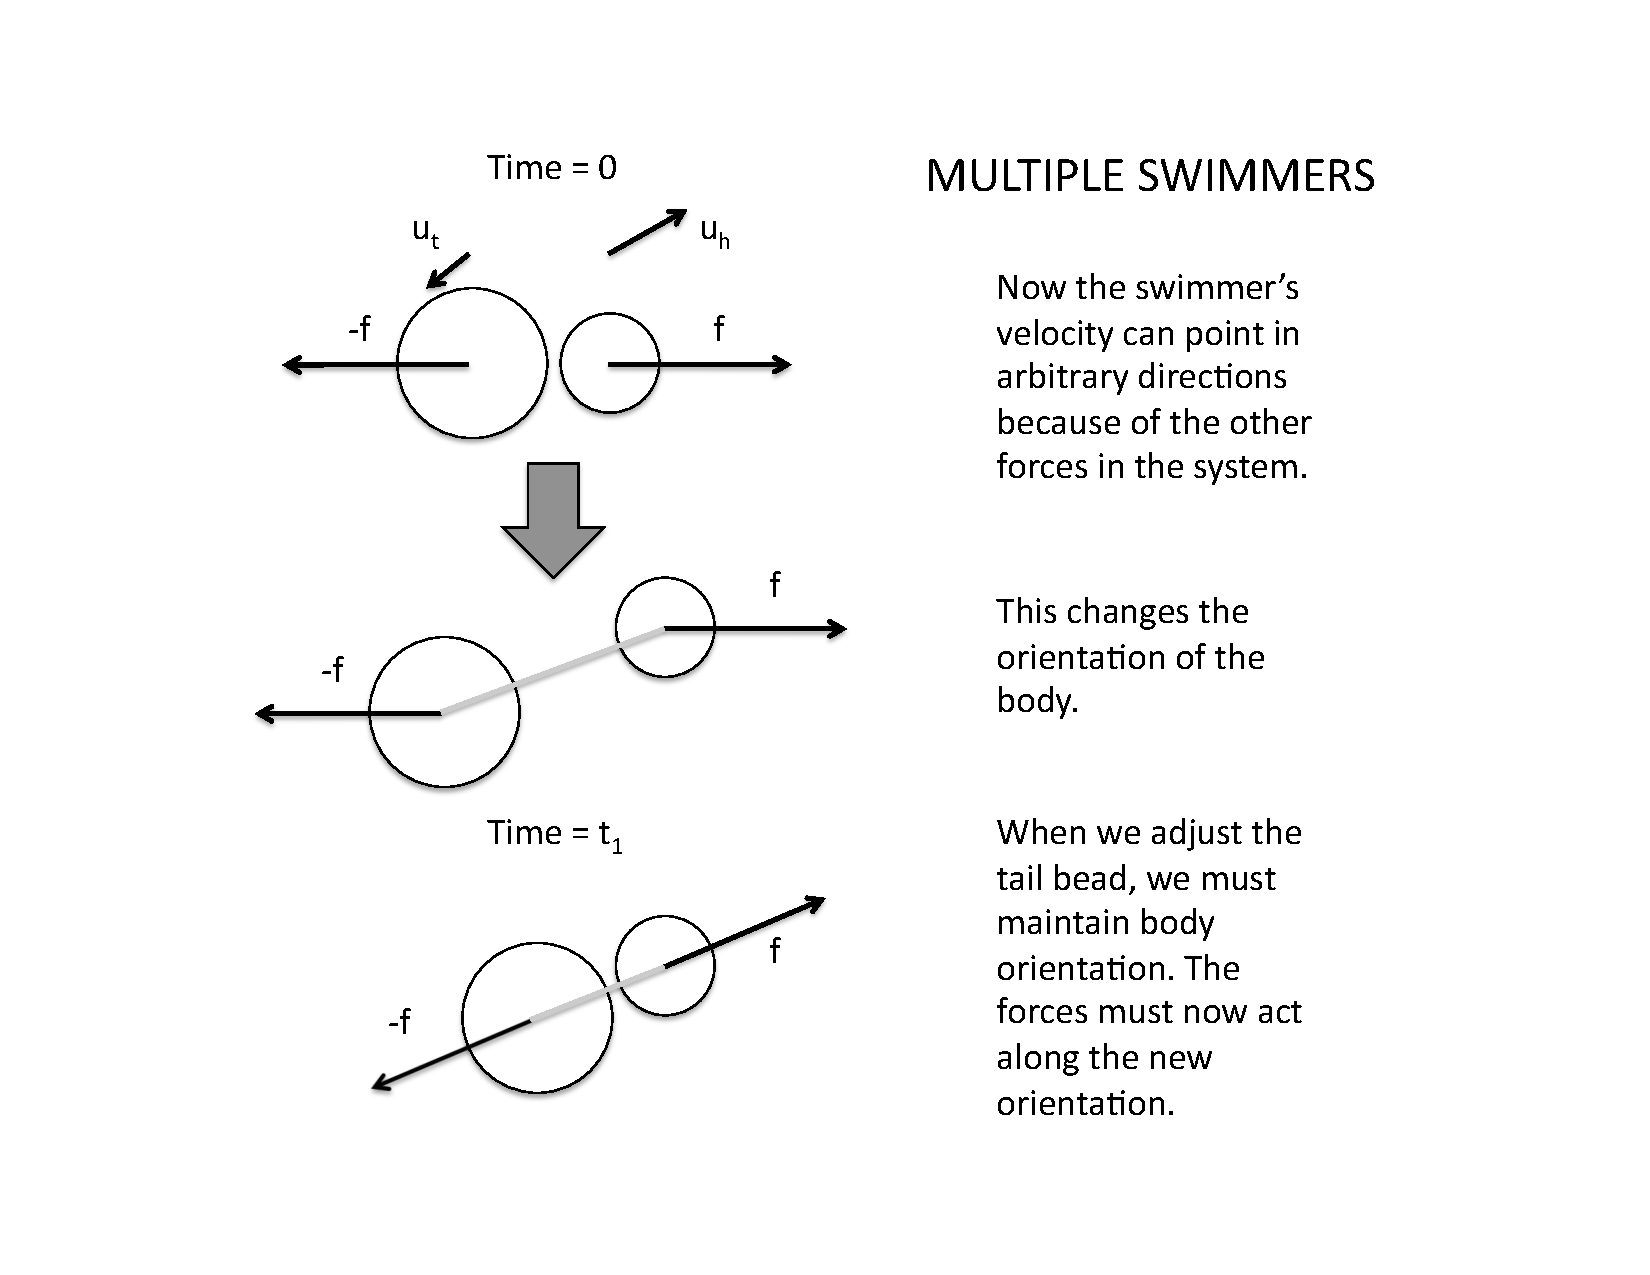
\includegraphics[width=6.5in]{MultipleSwimmers.pdf}
	\end{center}
	
	Because the body axis determines the direction of the forces, we really only have one parameter we can vary -- the magnitude of the forces. What can usually be measured about a microorganism is its speed. So let's say we have a choanoflagellate moving with speed $U$. How does this translate into a force?
	
	Recall for a single regularized Stokeslet that the velocity at the location of the Stokeslet is given by 
	\begin{equation*}
		\bu = \frac{H_1(0)}{\mu}\ff = \frac{1}{4\pi\mu\epsilon}\ff.
	\end{equation*}
	The velocity and the force point in the same direction, $\bv$. We know that $U$ is the (given) speed of the regularized Stokeslet and we let $F$ be the (unknown) magnitude of the force. Then we have
	\begin{equation*}
		U\bv = \frac{1}{4\pi\mu\epsilon}F\bv.
	\end{equation*}
	Since $\bv$ is the same vector, we have that the magnitude of the force is
	\begin{equation*}
		F = 4\pi\mu\epsilon	U.
	\end{equation*}
	
	With both a head point and a tail point modeling an organism, the situation is more complicated. Let's say that the head is moving with speed $U$. (Remember that we don't worry about the velocity of the tail.) Then the velocity at the head is influenced by both the forces at the head and at the tail, $F\bv$ and $-F\bv$ respectively. Also recall that the blob parameters for the head and the tail are different; we will call them $\epsilon_h$ and $\epsilon_t$. For simplicity, let's assume that the body orientation is in the x-direction, so that $\bx_h - \bx_t = (\ell, 0, 0)$ and $\bv = (1,0,0)$. This will be fine since we only need to find the magnitude of the force, not its direction in general. The velocity of the head is given by
	\begin{align*}
		\mu U\bv &= H_1(0,\epsilon_h)F\bv - \begin{pmatrix} H_1(\ell,\epsilon_t) + \ell^2 H_2(\ell,\epsilon_t) & 0 & 0 \\ 0 & H_1(\ell,\epsilon_t) & 0\\  0 & 0 & H_1(\ell,\epsilon_t) \end{pmatrix}F\bv \\ 
		\Rightarrow \mu U &= \frac{F}{4\pi\epsilon_h} - \frac{F}{4\pi\sqrt{\ell^2 + \epsilon_t^2}} \\
		\Rightarrow F &= \frac{4\pi\mu U}{\epsilon_h^{-1}-(\ell^2 + \epsilon_t^2)^{-1/2}}.
	\end{align*}
	
	This means that we can say that for a given force, we know how fast our swimmer is going in isolation. When there are many swimmers, of course the realized speed can be quite different. 
	
	We track the positions of the head of a choanoflagellate using the ODE
	\begin{equation*}
		\frac{d\bx_h}{dt} = \bu(\bx_h,t) = \frac{1}{\mu}M(\bx_h,\epsilon_h)\ff_h + \frac{1}{\mu}M(\bx_h,\epsilon_t)\ff_t,
	\end{equation*}
	where $M$ is the regularized Stokeslet matrix and $\ff_h$ and $\ff_t$ contain all the forces at the heads and tails of the choanoflagellates respectively. We use Euler's method for the time steps, so that $\bx_h^{n+1} = \bx_h^n + \Delta t \, \bu(\bx_h^n)$. We also must keep track of the orientation of the body. If the tail of the choanoflagellate was free to move away from the head, its new position would be $\bt = \bx_t^n + \Delta t \, \bu(\bx_t^n)$. Then the new body orientation is given by
	\begin{equation*}
		\bv = \frac{\bx_h^{n+1} - \bt}{|| \bx_h^{n+1} - \bt ||}.
	\end{equation*}
	
		
	
\end{document}